%part 4
%	\chapter{Изучение особенностей магнитооптической структуры синхротронов NICA и Nuclotron с учетом %ускорения поляризованных пучков и модернизация магнитооптической структуры Nuclotron с учётом возможности %изучения ЭДМ}\label{ch:EDM}

%	\chapter{Изучение особенностей магнитооптической структуры синхротронов для ускорения поляризованных пучков с учётом возможности изучения ЭДМ}\label{ch:EDM}
	\chapter{Возможности изучения ЭДМ легких поляризованных пучков заряженных частиц}\label{ch:EDM}
 
\par Известная проблема физики состоит в объяснении барионной асимметрии, то есть наблюдаемым преобладанием материи над антиматерией. До сих пор, существующие физические законы не способны полностью объяснить такой дисбаланс. В работе 1967 год А. Д. Сахаровым были сформулированы общие необходимые условия для наличия барионной асимметрии: 1) Нарушение закона сохранения барионного заряда; 2) Нарушение C- и CP-симметрии; 3) Нарушение на ранних этапах формирования Вселенной термодинамического равновесия \cite{sakharov}. Согласно второму условию, "\textit{Возникновение С-асимметрии по нашей гипотезе является следствием нарушения СР-инвариантности при нестационарных процессах расширения горячей Вселенной на сверхплотной стадии, которое проявляется в эффекте различия парциальных вероятностей зарядово-сопряженных реакций}".  Ранее в 1958 году С. Окубо теоретически показал такой эффект при рассмотрении распада сигма гиперона $\Sigma^{+}$ и его античастицы $\bar{\Sigma}^{+}$. Позднее в 1964 году Д. Кронин и В. Фитч экспериментально обнаружили нарушение CP-инвариантности слабого взаимодействия в процессах распада нейтральных каонов $K_{2}^{0}$ на два пиона $\pi^{+}, \pi^{-}$ \cite{CP}, за что в 1980 году были удостоены нобелевской премии по физике. 

\par В современной Стандартной модели частиц P- \cite{P-violation}и CP-симметрии нарушаются. Источником CP-нарушения является наличие комплексной фазы в матрице смешивания кварков Кабиббо-Кабаяси-Маскава для слабых взаимодействий \cite{CKM} и коэффициента $\theta_{\text{QCD}}$ в лагранжиане квантовой хромодинамики \cite{CPstrong}. Согласно CPT-теореме, CP-инвариантность эквивалентна T-инвариантности. Источником такого нарушения может являться ненулевой электрический дипольный момент (ЭДМ) элементарных частиц, который является фундаментальным свойством материи и обусловлен неоднородностью распределения заряда внутри частицы. Поскольку ЭДМ представляется полярным вектором, а не псевдовектором, то для него нарушается как P-, так и T-инвариантность, что показано на Рис. \ref{fig:4edmpt}.  Величина ЭДМ в Стандартной Модели слишком мала для экспериментального детектирования и находится на уровне $\abs{d_{n}}< 10^{-30}-10^{-32}$ $e\cdot \text{см}$ для нейтрона \cite{EMD_overview}. Возможность его существования была сформулирована в заметке 1950 Перселл и Рэмси \cite{EDM}, однако ненулевое ЭДМ пока точно не обнаружено. Другие теоретические модели, такие как Суперсимметричные (SUSY), также предсказывают наличие ЭДМ, но на уровне $\abs{d_{n}}< 10^{-27}-10^{-29}$ $e\cdot \text{см}$ для нейтрона, которые оставляют существенную надежду на экспериментальное обнаружение. Стоит отметить, что и таких точностей пока достигнуто не было, а сделаны только существенные ограничения для нейтрального нейтрона, впервые появившиеся в работе Н. Рамси и его коллег $\abs{d_{n}}< 5\times10^{-20}$ $e\cdot \text{см}$ ($90\%$ C.L.) \cite{NeutronEDM}, текущее ограничение находится на уровне $\abs{d_{n}}< 1.8\times 10^{-26}$ $e\cdot \text{см}$ ($90\%$ C.L.), что получено в работе nEDM \cite{neutron_EDM_current}.

\begin{figure}
	\centering
	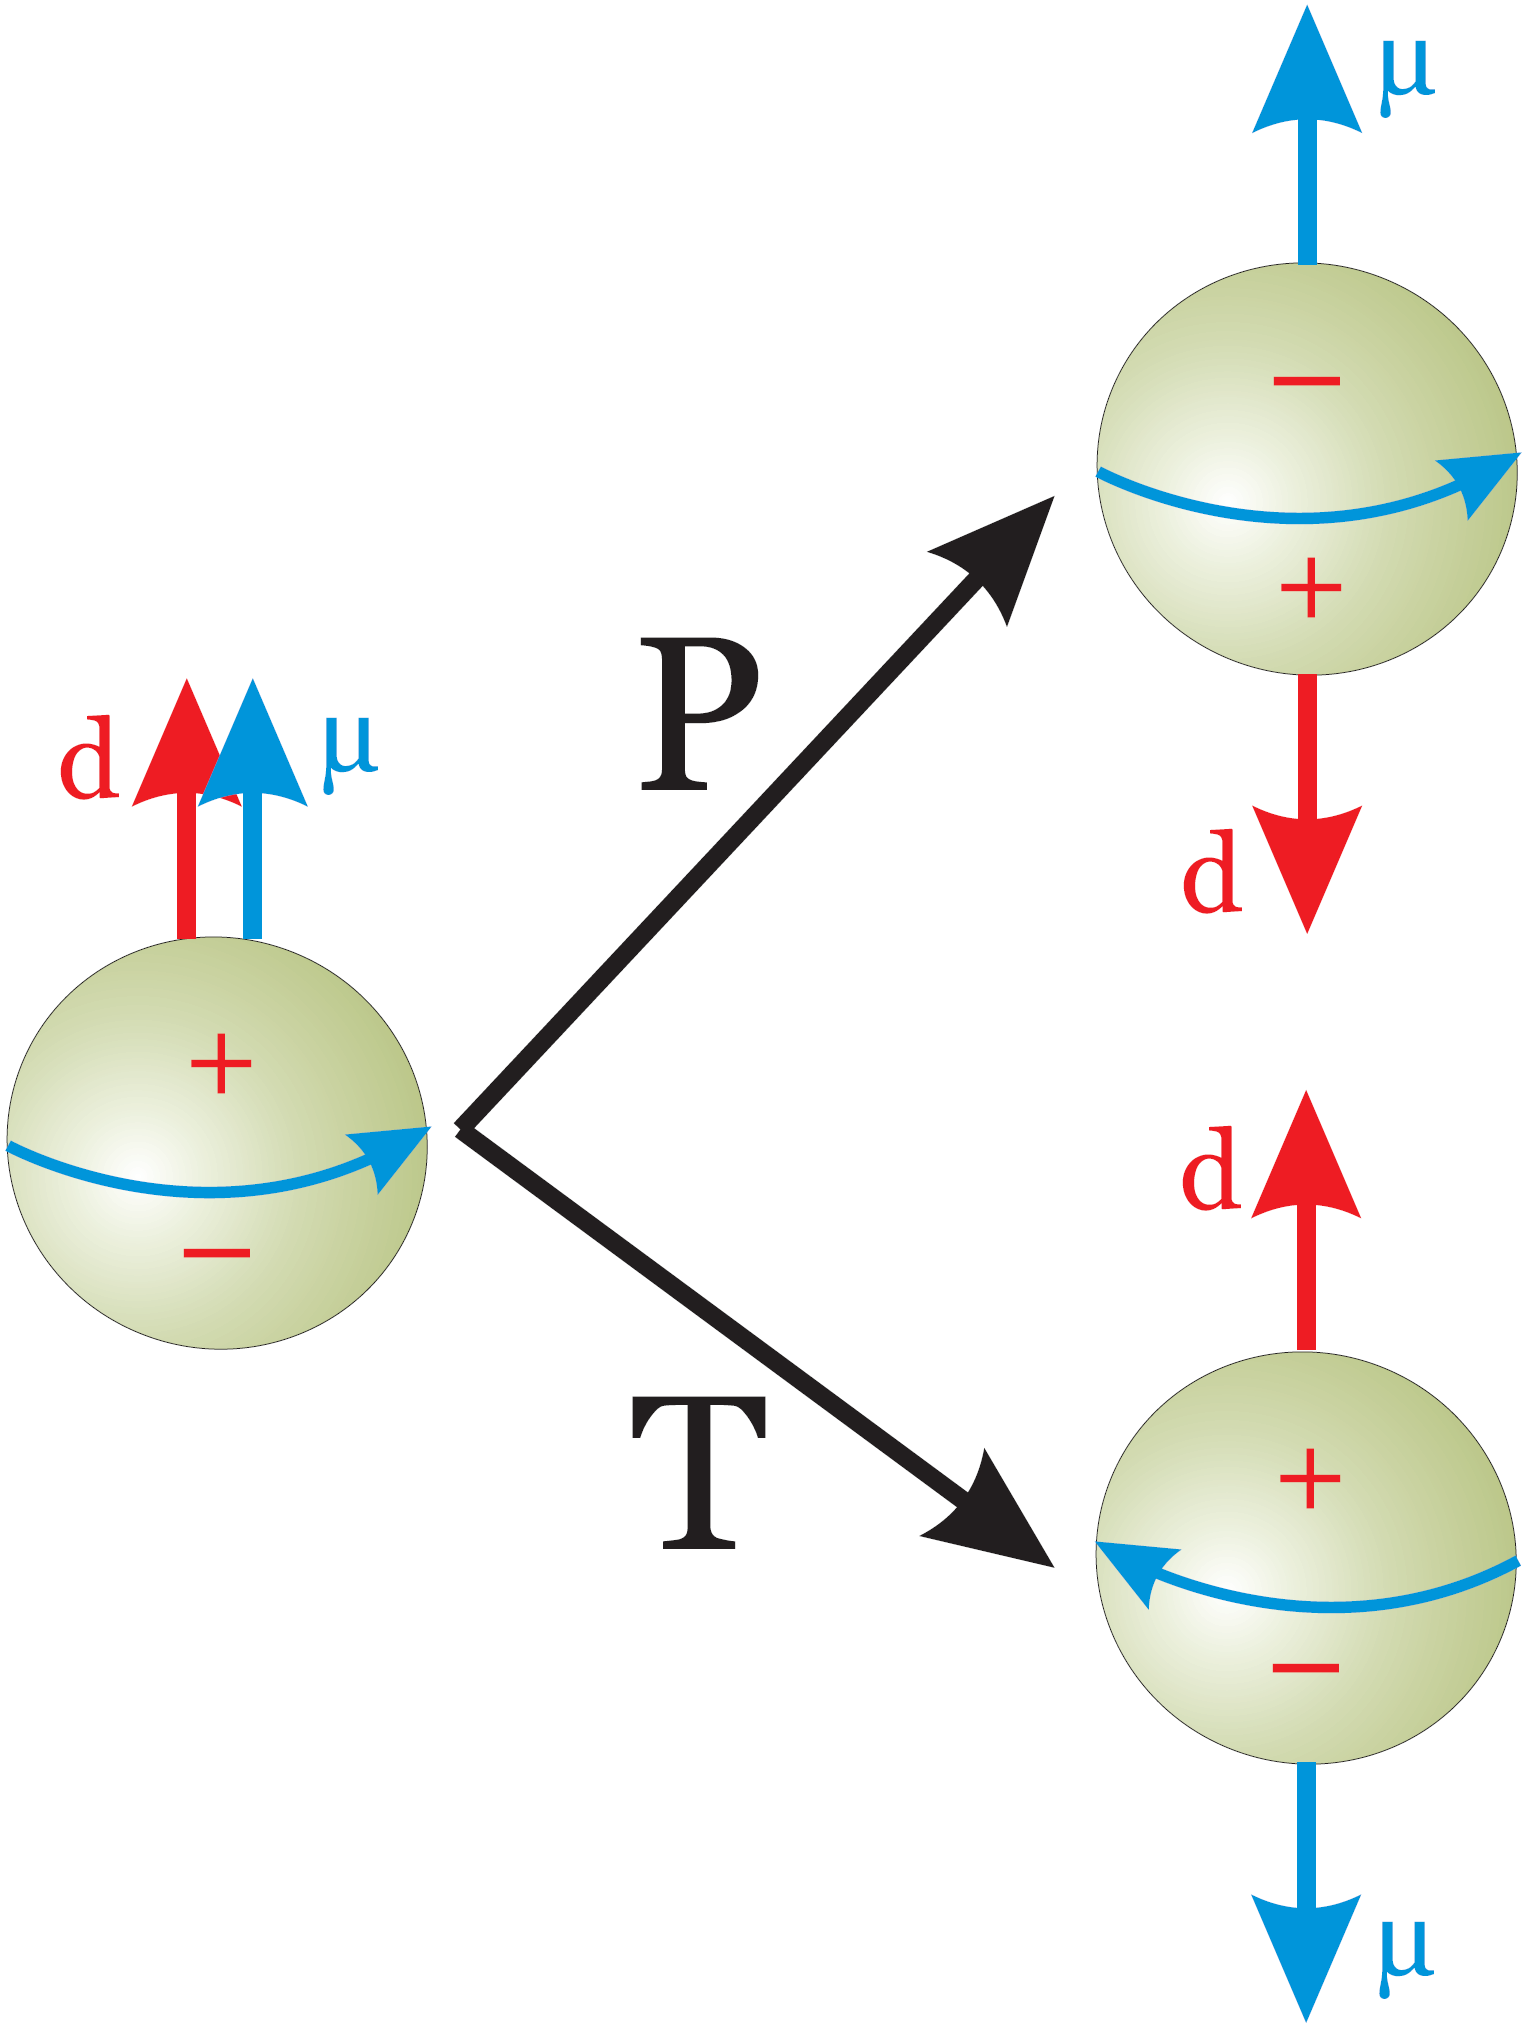
\includegraphics[width=0.3\linewidth]{images/4_EDM_P_T}
	\caption{Схематическое изображение нарушение P- и Т-симметрии ненулевым электрическим дипольным моментом.}
	\label{fig:4edmpt}
\end{figure}

\par Изучение ЭДМ нейтрона, а также нейтральных атомов удобно сохранением их положения при действии внешних магнитных и электрических полей. В случае заряженных частиц происходит движение, согласно силе Лоренца, что и приводит к необходимости применения ускорительных установок, позволяющих длительное накопление пучка с заданными параметрами и выступающих в роли накопительного кольца. Наиболее интересными и перспективными направлениями выглядит изучение ЭДМ протона и дейтрона. 

\par Обнаружение ЭДМ-эффекта может быть осуществлено по изучению поведения спина во внешних электромагнитных поля. Важным является отличие свойства индивидуальной частицы -- спина и пучка -- поляризации. Возможность изучения спина ансамбля частиц определяется теоремой Эренфеста \cite{Ehrenfest} и состоит в том, что уравнения для средних значений квантовых наблюдаемых величин формально тождественны уравнениям классической механики, если все величины заменить на соответствующие средние значения. Применение этой теоремы к чисто квантовой величине -- спин, позволяет оперировать понятием -- поляризации пучка, где усреднение осуществляется как по количеству частиц, так и по оборотам. Классическое уравнение описывающее эволюцию вектора спина было получено Телегди, Баргманн, Мишель в 1959 году \cite{TBMT}, с учётом одноименной прецессии Томаса. Вращение осуществляется за счёт наличия как магнитного дипольного момента (МДМ), так и ЭДМ 

\begin{align} \label{eq:T-BMT}
	\dv{{\vec{S}}}{t} &=\left(\vec{\Omega}_{\textrm{MDM}}+\vec{\Omega}_{\textrm{EDM}}\right) \times \vec{S}, \nonumber\\
	\vec{\Omega}_{\textrm{MDM}}&=-\frac{q}{m \gamma}\left\{(\gamma G+1)\vec{B}_{\perp}+(G+1)\vec{B}_{\parallel}-\left(\gamma G+\frac{\gamma}{\gamma+1}\right) \frac{\vec{\beta} \times \vec{E}}{c}\right\}, \\
	\vec{\Omega}_{\textrm{EDM}}&=-\frac{q \eta}{2 m}\left(\vec{\beta} \times \vec{B}+\frac{\vec{E}}{c}-\frac{\gamma}{\gamma+1}\frac{\vec{\beta}}{c}\left(\vec{\beta}\cdot\vec{E}\right)\right), \quad G=\frac{g-2}{2},\nonumber
\end{align}

\noindent где $\vec{\Omega}_{\textrm{MDM}}, \vec{\Omega}_{\textrm{EDM}}$ -- угловые частоты обусловленные наличием МДМ и ЭДМ; $q, m, G$ -- заряд, масса и магнитная аномалия; $\beta$ -- нормализованная скорость; $\gamma$ -- Лоренц-фактор; $d =~\eta \frac{q}{2mc}s$ -- ЭДМ фактор, $s$ -- спин. Уравнение содержит 2 слагаемых, одно обусловлено наличием МДМ, другое – ЭДМ соответственно \cite{silenko:edm}. Для непосредственного измерения ЭДМ-компоненты, влияние МДМ на спин должно быть нивелировано.

В текущий момент ведутся исследования поляризованных пучков в нескольких накопительных кольцах.

В кольце накопительного кольца COSY было получено время когерентности пучка SCT = 1000 секунд.

Новым крупным центром станет комплекс ОИЯИ NICA-Nuclotron в горде Дубна, Россия, с возможностью всестороннего изучения спиновой физики. В том числе уже упомянутое изучение ЭДМ заряженных частиц, коллайдерные эксперименты с симметричными и асимметричными пучками с целью изучения проблемы "спинового кризиса"\cite{ST_Filatov}, а также поиск аксиона \cite{Axion_Nikolaev}. В данной главе будут рассмотрены способы реализации квази-замороженного спина в периодических структурах и возможность их реализации 

Кроме того, частицы обладают магнитным дипольным моментом, который определяет взаимодействие с внешним магнитным полем.



\par Помимо, рассмотренного в Главах \ref{ch:dual}-\ref{ch:resonant}, коллайдера NICA, в ускорительный комплекс также входит установка Nuclotron \cite{nuclotron24}. Данный синхротрон предназначен как для самостоятельных экспериментов на выведенной мишени BM@N и изучения управления поляризацией, так и для использования в качестве инжектора поляризованного пучка протонов и дейтронов в коллайдер NICA. Однако, установка была введена в эксплуатацию в 90-е годы \cite{baldin:nuclotron} и может быть модернизирована с использованием новых современных магнитооптических элементов, производимых непосредственно в ОИЯИ г. Дубна \cite{korovkin:nica_magnets}. Для расширения возможностей Nuclotron в качестве самостоятельной машины рассматривается возможность изучения ЭДМ легких заряженных частиц. Такие прецизионные эксперименты возможны на ускорителе, работающем в режиме накопительного кольца с целью долгого удержания сгустка на орбите и накоплению достаточной статистики эксперимента. 

\par Возможность исследования ЭДМ с применением метода квази-замороженного спина возможна также и на установке, изначально для этого не предназначенной. Однако, поскольку для компенсации влияния МДМ необходимо использование элементов с электрическим полем, требуется дополнительное место для их расположение. Такое может быть достигнуто путем введения обводных каналов. Это возможно в том числе в кольце коллайдера NICA.

\par В экспериментах по измерению ЭДМ ключевым является обеспечение высокого показателя времени когерентности (SCT — Spin Coherence Time) порядка 1000 с \cite{AGSproposal}. В течение такого времени когерентный поляризованный пучок удерживается на орбите. Таким образом, для моделирования структуры с возможностью исследования ЭДМ необходимо гарантировать стабильность спиновой динамики вдоль всего кольца, что является отдельной задачей, наравне с обеспечением орбитальной стабильности пучка.

\section{Орбитальная и спиновая динамика в электромагнитных полях}\label{sec:EDM/requirements/deflector}

\par Рассмотрим как орбитальное, так и спиновое движение в электромагнитных полях. Для орбитального вращения в поперечном магнитном поле согласно уравнению Лоренца

\begin{equation} \label{eq:lorenz}
qc\vec{\beta}\times{\vec{B}}_\bot={\vec{\Omega}}_p^{\textrm{B}}\times\vec{p},
\end{equation}

\noindent где $q$ -- заряд, $c$ -- скорость света, $\vec{\beta}$ -- вектор относительной скорости, ${\vec{B}}_\bot$ -- поперечное магнитное поле, $\vec{p}$ -- импульс частицы, ${\vec{\Omega}}_p^{\textrm{B}}$ -- вектор угловой скорости (индексы означают, что происходит вращение импульса в магнитном поле). Учтем, что импульс частицы представим в виде $\vec{p}\ =\ \gamma mc\vec{\beta}$, тогда ур.\ref{eq:lorenz} с учетом перестановки векторного произведения получаем

\begin{equation}	
qc\vec{\beta}\times{\vec{B}}_\bot=-mc\gamma\vec{\beta}\times{\vec{\Omega}}_p^{\textrm{B}},
\end{equation}

\noindent для угловой скорости

\begin{equation} \label{eq:omega_pB}
 {\vec{\Omega}}_p^{\textrm{B}}=-\frac{q}{m\gamma}{\vec{B}}_\bot.
\end{equation} 

\begin{figure}[!h]
  \centering
	\includegraphics*[width=0.49\columnwidth]{4_orbital_B}
	\includegraphics*[width=0.49\columnwidth]{4_orbital_E}
   \caption{Вращение положительно заряженной частицы а) в магнитном поле; б) электростатическом поле.}
   \label{fig:4_orbital_B_E}
\end{figure}

\par Для заряженной частицы в электростатическом дефлекторе, выполняющего функцию поворота всегда соблюдается условие $\vec{p} \bot \vec{E}$, тогда происходит движение по окружности (рис.\ref{fig:4_orbital_B_E}) и аналогично ур.\ref{eq:lorenz}

\begin{equation}
q{\vec{E}}_\bot={\vec{\Omega}}_p^{\textrm{E}}\times\vec{p},
\end{equation} 

\noindent где ${\vec{E}}_\bot$ – электростатическое поле перпендикулярное импульсу, ${\vec{\Omega}}_p^{\textrm{E}}$ – вектор угловой скорости (индексы означают, что происходит вращение импульса в электростатическом поле)

\begin{equation}
q{\vec{E}}_\bot=mc\gamma{\vec{\Omega}}_p^{\textrm{E}}\times\vec{\beta}.
\end{equation} 

\noindent Для угловой скорости с учётом векторного произведения $\vec{v}=\vec{\omega}\times\vec{r}, \vec{\omega}=\frac{\vec{r}\times\vec{v}}{(\vec{r},\vec{r})}$

\begin{equation}
{\vec{\Omega}}_p^{\textrm{E}}=\frac{q}{mc}\frac{\vec{\beta}\times{\vec{E}}_\bot}{\gamma(\vec{\beta},\vec{\beta})}=\frac{q}{m\gamma}\frac{\vec{\beta}\times{\vec{E}}_\bot}{c\beta^2}\ \ \ 
\end{equation}

\par Рассмотрим теперь вращение спинового вектора под действием МДМ относительно вектора импульса

\begin{equation}
{\vec{\omega}}_p^{\textrm{B}}={\vec{\Omega}}_{\textrm{MDM}}^\textrm{B}-{\vec{\Omega}}_p^{\textrm{B}}=-\frac{q}{m\gamma}\left(\gamma G+1\right){\vec{B}}_\bot+\frac{q}{m\gamma}{\vec{B}}_\bot=-\frac{q}{m}{G\vec{B}}_\bot.
\end{equation}

\noindent Величина $\nu_s^{\textrm{B}}$ -- спин-тюн (spin-tune) является скалярной величиной и отражает во сколько раз поворот вектора спина больше поворота вектора импульса

\begin{equation} \label{eq:spintune_B}
\nu_s^{\textrm{B}}=\frac{\left|{\vec{\Omega}}_{\textrm{MDM}}^{\textrm{B}}-{\vec{\Omega}}_p^{\textrm{B}}\right|}{\left|{\vec{\Omega}}_p^{\textrm{B}}\right|}=\frac{-\frac{q}{m}{G\left|\vec{B}\right|}_\bot}{-\frac{q}{m\gamma}\left|{\vec{B}}_\bot\right|}=\gamma G.
\end{equation}

\noindent Аналогично для вращения в электростатическом поле
\begin{equation}
\begin{aligned}
{\vec{\omega}}_p^{\textrm{E}}={\vec{\Omega}}_{\textrm{MDM}}^{\textrm{E}}-{\vec{\Omega}}_p^{\textrm{E}}&=\frac{q}{m}\left(G+\frac{1}{\gamma+1}\right)\frac{\vec{\beta}\times\vec{E}}{c}-\frac{q}{mc}\frac{\vec{\beta}\times\vec{E}}{\gamma\beta^2} =\\
&=\frac{q}{mc}\left(G-\frac{1}{\gamma^2-1}\right)\vec{\beta}\times\vec{E}.
\end{aligned}
\end{equation}

\noindent Спин-тюн в электростатическом поле

\begin{equation} \label{eq:spintune_E}
\nu_s^{\textrm{E}}=\frac{\left|{\vec{\Omega}}_{\textrm{MDM}}^{\textrm{E}}-{\vec{\Omega}}_p^{\textrm{E}}\right|}{\left|{\vec{\Omega}}_p^{\textrm{E}}\right|}=\frac{\frac{q}{mc}\left(G-\frac{1}{\gamma^2-1}\right)\left|\vec{\beta}\times\vec{E}\right|}{\frac{q}{mc}\frac{\left|\vec{\beta}\times\vec{E}\right|}{\gamma\beta^2}}=\gamma\beta^2\left(G-\frac{1}{\gamma^2-1}\right).
\end{equation}
Примечательно, что спин-тюн как в магнитном поле ур.\ref{eq:spintune_B}, так и  электростатическом ур.\ref{eq:spintune_E} не зависит от величины поля в дефлекторе.

\section{Общий концепт квазизамороженной структуры}\label{sec:EDM/requirements/deflector}

\par Перейдем от рассмотрения общего случая вращения спина в магнитном и электрическом поле к непосредственным элементам и поворотным аркам. Из уравнений \ref{eq:spintune_B}, \ref{eq:spintune_E} видно, что для спиновой динамики сорт частиц существенно влияет на вращение относительно импульса. Для удобства повествования, все рассуждения и рисунки будут приведены для дейтрона, без потери общности, в дальнейшем будет рассмотрен и случай протонов.

\par Вращение в чисто магнитном кольце, содержащем в  поворотной арке только дипольные магниты, происходит под действием поперечного магнитного поля на $2\pi$, при этом поворот вектора импульса за один период осуществляется на $\Phi_p^{\textrm{arc}}=\sfrac{2\pi}{N}$, где $N$ – количество периодов, магнитных арок. Поворот спина, относительно спина происходит пропорционально $\gamma G$

\begin{equation}
\Phi_s^{\textrm{arc}}=\gamma G\cdot\Phi_p^{\textrm{arc}}.
\end{equation}

\begin{figure}[!h]
  \centering
	\includegraphics*[width=0.39\columnwidth]{4_arc_B}
	\includegraphics*[width=0.59\columnwidth]{4_arc_B+E}
   \caption{Отклонение спин-вектора в арке относительно импульса в случае дейтрона}
    \label{fig:4_arc_B_E}
\end{figure}

\noindent Принципиальная схема вращения импульса и спина пучка дейтронов показана для магнитной арке на рисунке \ref{fig:4_arc_B_E}a.

\par Рассмотрим простейший случай одного периода, состоящего из магнитной и электростатической арок, в котором может быть реализована компенсация МДМ-компоненты методом квази-замороженного спина. В отсутствии электростатических дефлекторов, вращение импульса в магнитной арке происходит на $\Phi_p^{\textrm{arc}}=\sfrac{2\pi}{N}$. При необходимости введения электростатической арки с отрицательной кривизной $\Phi_{p\textrm{E}}^{\textrm{def}}$, магнитные арки должны дополнительно поворачивать на угол $\Phi_{p\textrm{B}}^{\textrm{kick}}$ при помощи киккеров. Такой поворот будет впоследствие скомпенсирован поворотом в электростатической арке. На рис. \ref{fig:4_arc_B_E}б изображено поведения спин-вектора для дейтрона при последовательном действии магнитной арки, киккера, электростатической арки с отрицательной кривизной, киккера. Поворот импульса, после прохождения периода должен также быть повернуть на $\sfrac{2\pi}{N}$. Окончательно, 

\begin{equation}
\Phi_p^{\textrm{arc}}+\Phi_{p\textrm{B}}^{\textrm{kick}}+\Phi_{p\textrm{E}}^{\textrm{def}}=\frac{2\pi}{N}\ \ \
\end{equation}
или с учетом поворота в магнитной арке
\begin{equation}
\Phi_{p\textrm{B}}^{\textrm{kick}}={-\Phi}_{p\textrm{E}}^{\textrm{def}}\ \ \ 
\end{equation}


\noindent Спин-вектор в магнитной арке совершит отклонение в магнитном поле $\Phi_{s\textrm{B}}^{\textrm{arc+kick}}=\nu_s^{\textrm{B}}\left(\Phi_p^{\textrm{arc}}+\Phi_{p\textrm{B}}^{\textrm{kick}}\right)$. В электростатической арке $\Phi_{s\textrm{E}}^{\textrm{def}}=\nu_s^{\textrm{E}}\Phi_{p\textrm{E}}^{\textrm{def}}$. 
Отдельно для спинового движения, в киккерах и дефлекторе
\begin{equation}
\begin{aligned}
\Phi_s^{\textrm{kick+def}}  & = \nu_s^{\textrm{B}} \Phi_{p\textrm{B}}^{\textrm{kick}}+\nu_s^{\textrm{E}} \Phi_{p\textrm{E}}^{\text {\textrm{def}}}= \\
				& = \Phi_{p\textrm{B}}^{\textrm{kick}}\left[\gamma G-\beta^2 \gamma\left(G-\frac{1}{\gamma^2-1}\right)\right]= \\
				& = \Phi_{p\textrm{B}}^{\textrm{kick}}\left[\frac{G+1}{\gamma}\right]
\end{aligned}
\label{eq:spin_kick}
\end{equation}

\noindent Условие сохранения ориентации спин-вектора, то есть условие «квази-замороженности» можно записать в виде
\begin{equation}
\Phi_s^{\textrm{arc}}+\Phi_s^{\textrm{kick+def}}=0
\label{eq:QFS_condition}
\end{equation}

\noindent Тогда из уравнений \ref{eq:spin_kick} -- \ref{eq:QFS_condition} для 

\begin{equation} \label{eq:kick}
\Phi_{p\textrm{B}}^{\textrm{kick}}=-\Phi_p^{\textrm{arc}}\frac{\gamma^2G}{G+1}=-\frac{2\pi}{N}\frac{\gamma^2G}{G+1}\ \
\end{equation}

\noindent Отсюда видно, что кривизна дефлектора для дейтрона должна быть отрицательна, поскольку аномальный магнитный момент дейтрона отрицательный и меньше единицы $G_{\textrm{d}} = -0.142$.

\par Рассмотрим движение в прямом фильтре Вина. Ключевое условие -- равенство нулю силе Лоренца, таким образом фильтр Вина не отклоняет орбитальное движение
\begin{equation}
q\left(c\vec{\beta}\times{\vec{B}}_\bot+{\vec{E}}_\bot\right)=0.
\end{equation}
\noindent Стоит отметить, при этом выполняется равенство магнитного и электростатического абсолютных радиусов $\left|R_{\textrm{E}}\right|=\left|R_{\textrm{B}}\right|$ и для углов поворота
\begin{equation}
\Phi_{p\textrm{B}}^{\textrm{WF}}+\Phi_{p\textrm{E}}^{\textrm{WF}}=0\ \ \ 
\Phi_{p\textrm{B}}^{\textrm{WF}}=-\Phi_{p\textrm{E}}^{\textrm{WF}}=\Phi_p^{\textrm{WF}}.
\end{equation}

\noindent Поскольку импульс в фильтре Вина остается неизменным, то результирующее вращение спина может быть рассмотрено также относительно импульса. При этом необходимо подавить вращение от магнитной арки $\Phi_s^{\textrm{arc}}=\gamma G\cdot\Phi_p^{\textrm{arc}}$.
Таким образом условие «квази-замороженности» может быть записано аналогично ур. \ref{eq:QFS_condition} как 
\begin{equation}
\Phi_s^{\textrm{WF}}+\Phi_s^{\textrm{arc}}=0.
\end{equation}

\noindent Для спинового движения в фильтре Вина под действием МДМ выполняется

\begin{equation} \label{eq:spin_kick_WF}
\begin{aligned}
 \Phi_s^{\textrm{WF}} & =  \nu_s^{\textrm{B}} \Phi_{p\textrm{B}}^{\textrm{WF}}+\nu_s^{\textrm{E}} \Phi_{p\textrm{E}}^{\textrm{WF}}= \\
			& =  \Phi_p^{\textrm{WF}}\left[\gamma G-\beta^2 \gamma\left(G-\frac{1}{\gamma^2-1}\right)\right]= \\
			& =  \Phi_p^{\textrm{WF}}\left[\frac{G+1}{\gamma}\right]
\end{aligned}
\end{equation}

\noindent что совпадает с уравнением \ref{eq:spin_kick}. А значит и для угла поворота в фильтре Вина, аналогично ур. \ref{eq:kick}
\begin{equation}
\Phi_p^{\textrm{WF}}=-\Phi_p^{\textrm{arc}}\frac{\gamma^2G}{G+1}=-\frac{2\pi}{N}\frac{\gamma^2G}{G+1}.
\end{equation}

\par Такой результат говорит о том, что принципиальным для реализации квази-замороженности остается наличие отклоняющих полей. При использовании чисто электростатических дефлекторов, необходимо использовать дополнительный внешний магнитный толчок. В случае же прямого фильтра Вина используется скрещенные магнитное и электростатическое поля. Интегральная величина поля при этом сохраняется.

	\subsection{Длина компенсирующего элемента с электрической компонентой}\label{sec:EDM/requirements/length}
\par Радиус кривизны элемента с электрическим и магнитным полем может быть найден как
\begin{equation}
\begin{gathered}
\frac{1}{R}  = \frac{1}{R_\textrm{B}}+\frac{1}{R_\textrm{E}}, \ \ 
	R_\textrm{B}  = \frac{B\rho}{B}, \ \ 
	R_\textrm{E}  = \frac{\kappa}{E}, \ \ 
\end{gathered}
\end{equation}
где $B\rho=\sfrac{p_0}{e}$ – магнитная жесткость, $p_0=\gamma m\beta c$, $\kappa=\sfrac{p_0\beta c}{e}$ – электрическая жесткость.
Поскольку для фильтра Вина $R=\inf$, то и радиусы кривизны связаны $R_{\textrm{B}}=-R_{\textrm{E}}$. И для выбора радиуса достаточно определить либо магнитное поле, либо электрическое. Более строгое ограничение дается на электрическое поле $E_{\textrm{max}}=10\div13$ МВ/м.
Для нахождения длины
\begin{equation}
L={\Phi_p^{\textrm{WF}}R}_E=-\Phi_p^{\textrm{arc}}\frac{\gamma^2G}{G+1}R_E.
\end{equation}
Для минимальной длины в периодической структуре
\begin{equation} \label{eq:ele_length}
L_{\textrm{min}}=-\frac{2\pi}{N}\frac{\gamma^2G}{G+1}\frac{\kappa}{E_{\textrm{max}}}.
\end{equation}

	\subsection{Влияние сорта частиц на особенности спиновой динамики}\label{sec:EDM/requirements/particles}
	
\par В зависимости от сорта исследуемых частиц аномальный магнитный момент для протона $G_{\textrm{p}}=1.79$ и для дейтрона $G_{\textrm{d}}=-0.142$. Отличаются как абсолютное значение, так и знак. Если рассмотреть вывод формул, то всюду учитывалось, что введенные углы могут иметь как положительный, так и отрицательный знак. Таким образом уравнения могут быть использованы как для рассмотрения дейтрона, так и протона. 

\par  Как видно из рассмотренных структур, изучение одновременно ЭДМ дейтрона и протона в структуре с электростатическими дефлекторами не целесообразно по сравнению со структурой с использованием фильтров Вина. Во-первых, требуемая длина дефлекторов равна длине фильтров Вина, но в первом случае необходимы дополнительные киккеры. Во-вторых, кривизна дефлекторов для протонов и дейтронов имеет различный знак. В тоже время, фильтры Вина устанавливаются на прямой участок и не требуют альтернативного канала. А для изучения протонов фильтры Вина могут быть повернуты на 180 градусов относительно продольной оси. Использование дефлекторов может быть полезно в случае естественной способности орбитально отклонять пучок, что позволяет создать альтернативный канал.

	\subsection{Определение оптимальной энергии эксперимента}\label{sec:EDM/requirements/energy}
\par Как видно из Т-БМТ уравнения, зависимость от энергии пучка является определяющей для проведения эксперимента.  Эксперимент по исследованию ЭДМ не требует специального детектора, необходимо только наличие поляриметра. Такое устройство измеряет асимметрию рассеяния на образце. Это требование устанавливает энергию эксперимента и определяется потребностями поляриметрии. Для дейтрона, наибольшее сечение рассеяния на углеродной мишени находится при энергии пучка 270 МэВ (135 МэВ/нуклон) \cite{JEDI:polarimeter, skhomenko:polarimeter}.

\begin{figure}[!h]
  \centering
	\includegraphics*[width=0.7\columnwidth]{4_ele_length}
   \caption{Зависимость длины компенсирующего элемента в зависимости от энергии сгустка на нуклон}
   \label{fig:4_ele_length}
\end{figure}

\par Исходя из уравнения \ref{eq:ele_length}, рассмотрим как меняется длина используемого компенсирующего элемента от энергия эксперимента для протона и дейтрона. На рис. \ref{fig:4_ele_length} показано, что при оптимальной энергии $135$ МэВ/нуклон, длина элемента равна $L_{\textrm{d}} = 6.5$ м на период в случае дейтрона (суммарная необходимая длина на всей установке $L^{\textrm{total}}_{\textrm{d}} = 52$ м). Такая длина соответствует энергии $75$ МэВ для протонного пучка, при этом анализирующая способность поляриметра уменьшается в 3 раза \cite{mcnaughton:polarimeter} по сравнению с максимальной $L_{\textrm{p}} = 31$ м при $270$ МэВ. Таким образом, предложенная схема даёт большую надежду на изучение ЭДМ не только дейтрона, но и протона.
	
	\section{Использование Nuclotron в качестве бустера легких поляризованных частиц в коллайдер NICA}\label{sec:EDM/nuclotron}

\par Рассмотрим возможность использования синхротрона Nuclotron для ЭДМ исследований с применением концепции "квази-замороженного" спина.
\par В первую очередь, текущая структура Nuclotron может ускорять поляризованные протоны до энергии порядка $8$ ГэВ с возможной последующей инжекцией в коллайдер NICA для экспериментов на SPD детекторе при энергии $12.6$ ГэВ. Как было показано ранее в Главе \ref{ch:transition}, прохождение критической энергии без потерь в регулярной структуре при энергии $5.7$ ГэВ для протонного поляризованного пучка протонов является необходимым требованием коллайдерного эксперимента для достижения требуемой светимости. Таким образом, могут быть рассмотрены 2 вариации инжекции 1) ниже критической; 2) выше критической энергии коллайдера NICA. В первом случае, необходимо осуществить скачок критической энергии непосредственно в кольце коллайдера, что накладываются существенные ограничения на параметры пучка, в результате которых снижается светимость конечного эксперимента. Во втором случае, после инжекции необходимо охлаждение пучка при  при энергии 7-10 ГэВ. Однако, текущий электронный охладитель рассчитан на энергию пучка 2-3 ГэВ, что делает необходимым разработку новой установки электронного охлаждения.

\noindent В Главе \ref{ch:transition} был рассмотрен вариант модернизации модернизация кольца NICA с повышенной критической энергией. При таком подходе проблем с прохождением критической энергии не возникает, поскольку во всем диапазоне энергий вплоть до конечной энергии эксперимента критическая энергия не преодолевается. В этом случае инжекция может осуществляться на энергии $2-3$ ГэВ с эффективным электронным охлаждением на уже разработанной установке. Таким образом, максимальная энергия кольца Nuclotron может быть снижена без потери функции бустера.

	\section{Требвания к магнитооптической структуре синхротронов NICA-Nuclotron в задаче исследования электрического дипольного момента легких ядер}\label{sec:EDM/requirements}

Окончательно, при модернизации кольца Nuclotron должны быть учтены несколько факторов:

\begin{enumerate}
    \item Использование Nuclotron в качестве бустера поляризованных частиц в коллайдер NICA;
    \item Возможность проведения прецизионных экспериментов по исследованию ЭДМ заряженных частиц.
\end{enumerate}

\noindent Текущая структура Nuclotron не предполагает проведения экспериментов по исследованию ЭДМ. Рассмотрим возможные способы реализации такой программы как на текущей установке, так и возможные опции по модернизации. В первую очередь, рассмотрим необходимые требования с точке зрения спиновой динамики. Основным является требование скомпенсированности МДМ компоненты. Впервые, для достижения этого эффекта в BNL был предложен метод замороженного спина, в этом случае МДМ вращение равняется нулю для всего кольца. При таком подходе спин остается с всюду со-направлен с направлением импульса. Как можно увидеть из уравнений Т-БМТ, необходимо использование элементов со скрещенными магнитными и электрическим полями. 
Наличие чисто магнитных арок приводит к невозможности использовать метод заможенного спина для компенсации МДМ вращения спина. 

\par Альтернативным является метод квази-замороженного спина, в отличие от замороженного спина предполагает пространственное разделение электрического и магнитных полей и последовательная компенсация МДМ-компоненты. Компенсация может быть осуществлена на прямых участках с необходимостью использовать электрическое поле. Могут быть рассмотрены как чисто электростатические дефлекторы, так и фильтры Вина с перпендикулярными электрическим и магнитным полем.

\par Стоит отметить, что поскольку Nuclotron должен быть использован в качестве бустера в NICA, то необходимо реализовать структуру, работающую как для ускорения поляризованного протонного пучка до энергии порядка единицы ГэВ, так и низкоэнергетическую при энергии порядка сотен МэВ с возможностью изучения ЭДМ. Таким образом, ведущим полем должно выступать магнитное поле в поворотных магнитах, поскольку электрическое поле неспособно ускорить до энергии порядка единиц ГэВ. 

\par Отдельное внимание будет уделено критической энергии Нуклотрона. Она должна лежать выше максимальной энергии пучка.
	
	\section{Магнитооптика Nuclotron}\label{sec:EDM/optics}
	
\par В немодернизированной структуре Нуклотрона, расположение фильтров Вина полностью займёт всё пространство на прямых участках без возможности использования другого необходимого оборудования. Поэтому, рассмотрим возможность создания обходных каналов в исходной структуре. При таком подходе, оборудование можно расположить параллельно при наличии достаточного расстояния между полученными каналами.

\begin{figure}[!h]
  \centering
	\includegraphics*[width=0.99\columnwidth]{4_old_nuclotron}
   \caption{Твисс-функции текущей регулярной структуры Nuclotron.}
   \label{fig:4_old_nuclotron}
\end{figure}

\begin{figure}[!h]
  \centering
   \includegraphics*[width=0.49\columnwidth]{4_Nuclotron_original.png}
   \includegraphics*[width=0.49\columnwidth]{4_Nuclotron_original_def.png}
   \caption{Принципиальная схема расстановки структуры Nuclotron с текущей расстановкой элементов и с введением электростатических дефлекторов.}
   \label{fig:4_Nuclotron_original}
\end{figure}

\noindent На рис. \ref{fig:4_Nuclotron_original} показаны принципиальные схемы текущего синхротрона c пустыми прямолинейными промежутками $L_{\textrm{free}} = 7 \times 8 = 56$ м при использовании фильтра Вина и электростатического дефлектора. Максимальное расстояние между каналами может составить порядка $18$ см, чего недостаточно для параллельного расположения.

\par Таким образом, для увеличения длины прямых участков, может быть рассмотрена модернизация с оптимизацией диполей с магнитным полем $1.8$ Тл. Суммарная длина прямых промежутков должна составить $L_{\textrm{free}}+L^{\textrm{total}}_{\textrm{d}}=56+52 = 108$ м. Оставшееся место будет использовано как расстановки магнитных элементов, диполей, квадруполей, секступолей. Длина магнитной арки $L_{\textrm{arc}}=17.5$ м, а длина магнитов изменяется от 1.44 до 1.78 при этом их количество сокращается вдвое с $96$ до $48$. Тогда максимальная энергия протонного пучка может составлять $6.5$ ГэВ. Что удовлетворяет требованию использования Nuclotron в качестве бустера при $2-3$ ГэВ, а также возможности его использования на выведенной мишени экспериментов BM@N c понижением энергии от $10$ ГэВ до $6.5$ ГэВ \cite{kovalenko:nuclotron}. В случае фильтров Вина – они могут быть расположены в этом же канале последовательно, а для дефлекторов неизбежно должны быть реализованы дополнительные каналы.

\par Текущая структура Нуклотрона также неоптимальна с точки зрения ненулевой дисперсионной функции на прямых участках, что показано на рис. \ref{fig:4_old_nuclotron}.

	\subsection{Восьмипериодическая структура}\label{sec:EDM/optics/8period}

\par С учетом вышесказанного, была реализована восьмипериодическая структура на основе простейшей ФОДО ячейки. В такой структуре может быть применены обе опции подавления МДМ-компоненты: прямыми фильтрами Вина и электростатическами дефлекторами с киккер-магнитами.

\par В этом случае интересным является случай с использованием дефлекторов, тогда нет необходимости использовать прямые промежутки для нужд ЭДМ эксперимента. Дефлекторы могут быть расставлены как по краям, так и в центре рис. \ref{fig:4_Nuclotron_8}, при этом расстояние между каналами составляет $47$ и $50$ см соответственно.

\par Подавление дисперсии может быть осуществлено выбором кратного количества набега фазы $\nu_x,y = 1$. Стоит отметить, что наличие электростатики при энергии $E_{\textrm{edm}}=270$ МэВ, искажает дисперсию, которая не компенсируется магнитным полем. Однако, она может быть долнительно компенсирована квадруполями арки, при этом набега фазы также искажается.

\begin{figure}[!h]
  \centering
   \includegraphics*[width=0.49\columnwidth]{4_Nuclotron_8_def1.png}
   \includegraphics*[width=0.49\columnwidth]{4_Nuclotron_8_def2.png}
   \caption{Принципиальная схема расстановки восьмипериодической структуры Nuclotron с текущей расстановкой при введении электростатических дефлекторов.}
   \label{fig:4_Nuclotron_8}
\end{figure}

\begin{figure}[!h]
  \centering
   \includegraphics*[width=1\columnwidth]{4_Nuclotron_twiss_8}
   \caption{Твисс-функции регулярной поворотной арки восьмипериодической модернизированной структуры Nuclotron.}
   \label{fig:4_Nuclotron_twiss_8}
\end{figure}

\begin{figure}[!h]
  \centering
   \includegraphics*[width=1\columnwidth]{4_Nuclotron_Def_twiss_8}
   \caption{Твисс-функции регулярной поворотной арки восьмипериодической модернизированной структуры Nuclotron с дефлекторами.}
   \label{fig:4_Nuclotron_Def_twiss_8}
\end{figure}

\newpage
	\subsection{Модернизированная 16-периодическая структура}\label{sec:EDM/optics/16period}

\begin{figure}[!h]
  \centering
   \includegraphics*[width=0.5\columnwidth]{4_Nuclotron_16.png}
   \caption{Принципиальная схема расстановки восьмипериодической структуры Nuclotron с текущей расстановкой при введении электростатических дефлекторов.}
   \label{fig:4_Nuclotron_16}
\end{figure}

\begin{figure}[!h]
  \centering
   \includegraphics*[width=1\columnwidth]{4_Nuclotron_twiss_16.png}
   \caption{Твисс-функции 16-периодической модернизированной структуры Nuclotron без фильтров Вина.}
   \label{fig:4_Nuclotron_twiss_16}
\end{figure}

\begin{figure}[!h]
  \centering
   \includegraphics*[width=1\columnwidth]{4_Nuclotron_WF_twiss_16.png}
   \caption{Твисс-функции 16-периодической модернизированной структуры Nuclotron c фильтрами Вина.}
   \label{fig:4_Nuclotron_twiss_16}
\end{figure}

\par С целью увеличения точности проведения эксперимента, "квази-замороженный" спин может быть как можно больше приближен к режиму "замороженного" спина. Изменяя периодичность структуры, изменяется и угол отклонения спина на каждом периоде, уменьшение ЭДМ сигнала происходит согласно формуле $J_0\left(\Phi_s\right) \approx 1-\frac{\left(\Phi_s\right)^2}{4}$  \cite{Senichev:2023_nuclotron}. 

\par Для этого магнитная арка, соответствующая рассмотренному случаю восьмипериодической структуры, может быть раздвинута для создания дополнительного прямого промежутка, однако такой подход нарушает регулярность и соответствующая структура должна быть рассмотрена как резонансная.

\par Стоит отметить, что 16-ти периодической эта структура называется именно по причине возможности разделения фильтров Вина на большее количество, делая угол отклонения спина меньше двое, по сравнению с приведенной выше структурой. Однако, по своей сути, структура имеет периодичность равную 8.

\par С точки зрения построения магнито-оптической структуры модернизированного Нуклотрона следовали нескольким целям. Во-первых, как мы видим суперпериод построен таким образом, чтобы в центральной ячейке было дрейфовое пространство без поворотных магнитов, в том месте, где дисперсионная функция имеет максимальное значение при бесконечном значении кривизны траектории, что позволит поднять критическую энергию. Во-вторых, число суперпериодов равное восьми, незначительно превышает частоту бетатронных колебаний ${\nu}_x$ в горизонтальной плоскости, что облегчает регулировку коэффициента уплотнения орбиты. В-третьих, введение центрального дрейфа упрощает размещение трех семейств секступолей, необходимых для регулирования бетатронной и спиновой хроматичностей, в то время, как боковые дрейфовые участки удобны для размещения фильтров Вина. И наконец, максимальное значение дисперсии в центре суперпериода совпадает с минимальным значением горизонтальной $\beta_x$ функции.



\begin{equation}
\begin{array}{|l|l|l|l|l|l|l|l|l|}
\hline \text { структура } & \text { Длина } & \text { число } & \text { Общая } & \text {, Тесла } & \text { Т м } & \text { Макс } & \text { нуклон } & \text { протон } \\
\hline \text {Nuclotron} & 1.44 & 96 & 138.24 & 1.8 & 39.6 & 10.14 & 5.07 & 10.97 \\
\hline \text {Nuclotron 2.1} & 2.35 & 48 & 112.77 & 1.8 & 32.2 & 8 & 4 & 8.79 \\
\hline \text {Nuclotron 2.2.1 } & 1.78 & 48 & 85.3 & 1.8 & 24.4 & 5.7 & 2.85 & 6.47 \\
\hline \text {Nuclotron 2.2.2} & 1.78 & 48 & 85.44 & 1.8 & 24.5 & 5.7 & 2.85 & 6.47 \\
\hline \text {Nuclotron 2.2.3} & 2.10 & 48 & 101 & 1.8 & 28.93 & 7.0 & 3.5 & 7.8 \\
\hline
\end{array}
\end{equation}

	\subsection{Предпосылки модернизации главного кольца NICA}\label{sec:EDM/Wien_filter/modernization}

\par Для изучения ЭДМ в кольце коллайдера NICA возможно только использование концепции "квази-замороженного" спина, поскольку поворотные арки являются чисто магнитными. Кроме того, коллайдерная мода использует всё пространство прямых промежутков, а также имеет точки соударения. Для решения обоих указаных проблем, могут быть созданы обходные каналы, в которых будут расположены прямые фильтры Вина. Таким образом, возможно использовать главного кольца NICA в качестве накопителя, а не в режиме коллайдера. Создание обводных каналов является большим преимуществом, не требующим значительной перестройки комплекса и затрат, при всём при этом, позволяющим задействовать NICA в различных экспериментах.

\par Приведенные ранее особенности являются решающими при выборе энергии эксперимента и сорта частиц. В будущем вся предлагаемая магнитооптика будет рассмотрена для дейтронов с энергией $240$ МэВ. Стоит отметить, что расчеты показывают основные параметры магнитного поля диполей $B_{\textrm{dip}}=0.132$ Т, а также магнитную жесткость $B\rho=3.252 \ \textrm{T} \cdot$м.

\par Проектируя накопительное кольцо NICA с обводными секциями ByPass, планируется, оставить геометрию арок неизменной. Возможно лишь изменение полей в уже установленных элементах. Так чтобы NICA можно было использовать для различных экспериментов.

\par В кольце NICA, арка имеет ненулевую дисперсию. По краям как дисперсия, так и ее производная сведены к нулю. Прямой участок имеет нулевую дисперсию по всему периметру. Общая длина оригинального кольца NICA $L_{\textrm{acc}}=503.04$ м. Длина одной арки равна $L_{\textrm{arc}}=142.15$ м. Итак, доступно $\left(L_{\textrm{acc}}-2L_{\textrm{arc}}\right)/2=109.6$ м. 
\par ByPass – обводной канал с альтернативной прямой секцией, не содержащее место встречи. Дипольные магниты выбраны таким образом, чтобы обеспечить отклонение на угол $\alpha=\ 9$. Сила диполя $B_{\textrm{BP}}=1$ Т при длине $L_{\textrm{dip}}^{\textrm{BP}}=50$ см. Альтернативный прямой участок находится на расстоянии $1$ м от исходного, поэтому длина обводного участка $L_{\textrm{BP}}=1\mathrm{м/sin\alpha}\sim6.4$ м. Принципиальная схема обходных каналов показана на рисунке \ref{fig:4_NICA_bypass}.

\begin{figure}[!h]
  \centering
   \includegraphics*[width=1.0\columnwidth]{4_NICA_bypass.png}
   \caption{Принципиальная схема обходных каналов ByPass в существующем комплексе NICA.}
   \label{fig:4_NICA_bypass}
\end{figure}

\par Отклоняющие магниты искажают дисперсионную функцию. Таким образом, необходимо было использовать по меньшей мере 2 фокусирующих квадруполя на обходном канале для подавления дисперсия на выходе. Это поможет обеспечить нулевую дисперсию на всем прямолинейному участке. Чтобы обеспечить периодичность и симметрию бета-функций, можно использовать или один или три дефокусирующих квадруполя.
\par Будут рассмотрены два случая, с адаптированными прямыми участками, идентичным поворотным аркам, но без магнитов. Это сделано для простоты моделирования в регулярной идеальной структуре. Наконец, мы рассмотрим реальный случай магнитооптики с полностью регулярной ФОДО прямой секцией.

\subsubsection{Первичная схема с 3 квадруполями}\label{sec:EDM/Wien_filter/ByPass/3quad}

\par В этом случае байпас состоит из минимально возможных 3 квадруполей: 2 фокусирующих QBP1 и 1 дефокусирующий QBP2 (рис. \ref{fig:4_bypass_3scheme}). Согласование арки с каналом ByPass обеспечивается тремя квадруполями QM1, QM2, QM3 (секция согласователя Matching M1). А согласование ByPass с прямым участком также симметрично осуществляется такими же квадруполями QM1, QM2, QM3. Это возможно в силу изначально заложенной симметрии между аркой и прямым участком. Тогда общая длина всего ускорителя составит $L_{\textrm{3quad}}^{\textrm{acc}}=503.46$ м.
\par На рисунке \ref{fig:4_bypass_3quad} приведены Твисс-функции, черными линиями указаны границами канала ByPass. Максимум бета-функции $\beta_y$ расположен в центре канала ByPass. И может принимать большое значение, по сравнению с $\beta_{x}$. По этой причине можно рассмотреть случай с 5 квадруполями в отводном канале.

\begin{figure}[!h]
  \centering
   \includegraphics*[width=1.0\columnwidth]{4_bypass_3scheme.png}
   \caption{Принципиальная схема ByPass с 3 квадруполями.}
   \label{fig:4_bypass_3scheme}
\end{figure}

\begin{figure}[!h]
  \centering
   \includegraphics*[width=1.0\columnwidth]{4_bypass_3quad}
   \caption{Twiss-параметры для ByPass с 3 квадруполями. Черными линиями показано расположение дефлекторов.}
   \label{fig:4_bypass_3quad}
\end{figure}

\subsubsection{Схема ByPass с 5 квадруполями}\label{sec:EDM/Wien_filter/ByPass/5quad}

\par По сравнению с предыдущим случаем, обводной канал состоит из 5 квадруполей, которые представлены 2 семействами: фокусирующим QBP1 и дефокусирующим QBP2. Он становится длиннее $L_{\textrm{5quad}}^{\textrm{BP}}=9.35$ м и отклоняется на $1.46$ м (рис. \ref{fig:4_bypass_5scheme}). Теперь секции согласования M1 и M2 по-прежнему идентичны, но представлены двумя квадруполями QM1 и QM2 для обеспечения регулярности Твисс-функций. Однако, полная длина ускорителя становится больше, NICA $L_{\textrm{5quad}}^{\textrm{acc}}=510.02$ м. На рисунке \ref{fig:4_bypass_5quad} показаны, что максимум $\beta_y$ становится меньше в центре. Стоит отметить, что максимум дисперсионной функции стал увеличился от $D_x^{\textrm{3quad}} \sim 0.2$ м до $D_x^{\textrm{5quad}} \sim 0.5$ м. Таким образом, этот случай должен быть адаптирован к реальному.

\begin{figure}[!h]
  \centering
   \includegraphics*[width=1.0\columnwidth]{4_bypass_5scheme.png}
   \caption{Принципиальная схема ByPass с 5 квадруполями.}
   \label{fig:4_bypass_5scheme}
\end{figure}

\begin{figure}[!h]
  \centering
   \includegraphics*[width=1.0\columnwidth]{4_bypass_5quad}
   \caption{Twiss-параметры для ByPass с 5 квадруполями. Черными линиями показано расположение дефлекторов.}
   \label{fig:4_bypass_5quad}
\end{figure}

\subsubsection{Адаптированный вариант}\label{sec:EDM/Wien_filter/ByPass/final}

\par Основываясь на рассмотренных примерах, наконец, можно получить структуру, максимально адаптированную к реальным длинам установки. Теперь рассмотрим полностью регулярный прямой участок, который стал короче $L_{\textrm{SS}}^{\textrm{BP}}=80.71$ м (рис. \ref{fig:4_bypass_real_scheme}). Байпас состоит из 5 квадруполей и отклоняет пучок на $1.46$ м. Но для согласования использовались разные секции M1 и M2, чтобы компенсировать не симметрию между поворотной аркой и прямым участком. Наконец, Твисс-функция половины байпасного NICA, представлена на рисунке \ref{fig:4_bypass_twiss_ring}. В центре прямой секции расположены фильтры Вина. Все расчеты выполнены при помощи программ OptiM \cite{optim} и COSY Infinity \cite{cosy}.

\par Для экспериментов с ЭДМ необходимо использовать NICA в качестве накопительного кольца. По этой причине была рассмотрена модернизация путем создания альтернативных прямых участков, параллельных исходным, с использованием каналов ByPass. Также на прямых участках есть возможность разместить специальные элементы – фильтры Wien для компенсации вращения спина от МДМ компоненты в поворотных арках. Поскольку арки остаются неизменными, это позволяет использовать NICA в различных экспериментах.
\par Рассмотрены 2 принципиальные схемы обходного канала. И, наконец, получили наиболее реалистичный случай, когда прямой участок полностью регулярный. Конечная конструкция удовлетворяет всем необходимым требованиям к магнитооптике. Исследование спин-орбитальной динамики с оптимизированными фильтрами Вина показывают, спин восстанавливает ориентацию на прямом участке и метод "квази-замороженного" спина может быть реализован в ByPass NICA.

\begin{figure}[!h]
  \centering
   \includegraphics*[width=1.0\columnwidth]{4_bypass_real_scheme.png}
   \caption{Принципиальная схема адаптированной структуры кольца NICA c ByPass.}
   \label{fig:4_bypass_real_scheme}
\end{figure}

\begin{figure}[!h]
  \centering
   \includegraphics*[width=1.0\columnwidth]{4_bypass_twiss_ring.png}
   \caption{Twiss-функции для половины адаптированной структуры кольца NICA c ByPass. Фильтры Вина, расположенные на прямом участке.}
   \label{fig:4_bypass_twiss_ring}
\end{figure}

\newpage
\section{Спин-орбитальная динамика пучка в фильтрах Вина, спин-орбитальный трекинг в магнитном кольце со скрещенными E+B элементами} \label{sec:EDM/Wien_filter_tracking}

\par Стоит особо отметить, что спин разных частиц, из-за их движения в трехмерном пространстве, в любом случае, прецессирует со слегка отличающимися частотами вокруг инвариантной оси. Таким образом, нарушает спиновую когерентность. Для обеспечения спиновой когерентности необходимо использовать нелинейные элементы, секступоли, расположенные в местах с ненулевой дисперсией, на поворотных арках. Так как секступоли также влияют и на бетатронную хроматичность, мы рассматриваем возможность одновременного подавления обоих эффектов.

\subsection{Декогеренция спина}\label{sec:EDM/Wien_filter_tracking/decoherence}

Следствием уравнения Т-БМТ (1) является частота вращения спина в электрическом и магнитном полях и задаются выражениями:

\begin{equation}
\begin{aligned}
\nu_{s}^{B} &= \gamma G \\
\nu_{s}^{E} &= \frac{G+1}{\gamma}-G \gamma
\end{aligned}
\end{equation}

\par Равновесный уровень энергии частицы

\par Разные частицы имеют различный импульс, и существует необходимость в использовании понятия эффективной энергии:

\begin{equation}
\gamma_{eff}=\gamma_s+\beta_s^2\gamma_s\Delta\delta_{eq}
\end{equation}

\par Распределение равновесного импульса из-за бетатронного движения и ненулевого коэффициента уплотнения импульса второго порядка основано на синхронном принципе [4] и определяется с помощью:

\begin{equation}
\Delta\delta_{eq}=\frac{\gamma_s^2}{\gamma_s^2\alpha_0-1}\left[\frac{\delta_0^2}{2}\left(\alpha_1+\frac{3}{2}\frac{\beta_s^2}{\gamma_s^2}-\frac{\alpha_0}{\gamma_s^2}+\frac{1}{\gamma_s^4}\right)+\left(\frac{\Delta L}{L}\right)_\beta\right]
\end{equation}

\noindent для определения удлинения орбиты из-за бетатронных колебаний:

\begin{equation}
\left(\frac{\Delta L}{L}\right)_\beta=-\frac{\pi}{L_0}\left[\epsilon_x\nu_x+\epsilon_y\nu_y\right],
\end{equation}

\noindent где индекс s означает синхронную частицу, $\epsilon_x$, $\epsilon_y$ – эмиттансы, $\nu_x$, $\nu_y$ – частота бетатронных колебаний, $\delta_0$ – относительный разброс импульса, $\alpha_0$, $\alpha_1$ – два первых порядка коэффициента уплотнения импульса. Уравнение 2 вместе с Уравнениями (3-5) показывают, что разброс спиновой частоты зависит от равновесного уровня энергии частицы.

\textbf{Удлинение орбиты и бетатронная хроматичность}

\par Более формальная теория подразумевает воздействие внешнего (секступольного) поля. Принимая во внимание выражение для полного удлинения орбиты из [5]:

\begin{equation}
\Delta C_\Sigma=-2\pi\left(J_x\xi_x+J_y\xi_y\right)+\delta_0\left(\alpha_0+\alpha_1\delta_0+\alpha_2\delta_0^2+\ldots\right),
\end{equation}

где $\xi_x$, $\xi_y$ – хроматичности. Если мы сравним Уравнение 6 с Уравнениями 4, 5 можно заметить, что длина орбиты тесно связана с равновесным уровнем энергии.

\subsection{Секступольная коррекция}\label{sec:EDM/Wien_filter_tracking/sextupole_correction}

\par В результате Уравнения 4, 6 показывают, что использование секступолей может влиять на частоту прецессии спина $\nu_s$ и в конечном счёте позволяют достигнуть спиновой когерентности. Такие эксперименты были проведены на ускорителе COSY в Юлихе, Германия, чтобы получить время когерентности (Spin Coherence Time) SCT на уровне $1000$ секунд [6]. Секступоли располагаются в местах с ненулевой дисперсией на поворотных арках. В минимумах и максимумах дисперсионной $D_{x,y}$ и бета $\beta_{x,y}$ функциях оказывают наибольшее воздействие и физически располагаются рядом с квадрупольными линзами. Твисс-функции арки NICA являются регулярными и показаны на Рисунке 1 [7].

\begin{figure}[!h]
  \centering
   \includegraphics*[width=1.0\columnwidth]{4_NICA_arc.png}
   \caption{Twiss-параметры ByPass NICA для дейтронного режима в OptiM. Также показано расположение секступольных семейств.}
   \label{fig:4_NICA_arc}
\end{figure}

\textbf{Бетатронная хроматичность}
Для коррекции бетатронной хроматичности используется только 2 семейства секступолей: одно вблизи фокусирующих квадруполей, другое – рядом с дефокусирующими. Натуральная хроматичность накопительного кольца ByPass NICA равна $\nu_{x,y}=-17/-17$. После оптимизации можно отслеживать частоту прецессии спина на Рисунке 2: красная линия показывает натуральную хроматичность, синяя – скорректированную, подавленную до нуля. Для этого случая также был осуществлен спин-трекинг в течение $3\times{10}^6$ оборотов для частиц с различным начальным отклонением в координатах $x, y, d$ с начальной ориентацией спина ${\vec{S}}_0$ под углом $45$ градусов в плоскости $y-z$, что показано на Рисунке 3 [8].

\begin{figure}[!h]
  \centering
   \includegraphics*[width=1.0\columnwidth]{4_spin_decoherence.png}
   \caption{Спиновый трексинг частиц с различным начальным отклонением в координатах x, y, d с использованием 2 семейств секступолей для получения нулевой бетатронной хроматичности.}
   \label{fig:4_spin_decoherence}
\end{figure}

\textbf{Спиновая когерентность}
\par Чтобы достигнуть спиновой когерентности, рассмотрим чисто частоту прецессии спина. COSY Infinity \cite{cosy} не может работать вблизи нулевого значения частоты прецессии спина. Так как это может привести к ошибке из-за резонанса, по этой причине отстраиваемся от резонанса до уровня $\nu_s~{10}^{-4}$. Но к частицам предъявляется требование прецессировать синхронно — когерентно. 
Основным параметром является частота вращения спина, которая в общем случае зависит от координат и энергии. Можно видеть, что доминирующим компонентом является квадратичный член в разложении частоты спиновой прецессии. Это видно на Рисунке 2 для обоих случаев – как для натуральной хроматичности, так и скорректированной хроматичности. По этой причине секступоли могут быть выбраны другим способом, чтобы просто достигнуть спиновой когерентности.
Как мы можем видеть из Уравнений 4, 6, недостаточно использовать 2 семейства, таким образом, третье семейство должно быть использовано для подавления зависимости от энергетической компоненты. Но в регулярных структурах бета и дисперсионные $\beta$, $D$ - функции не позволяют использовать 3 линейных независимых семейства. На Рисунке 1 показано расположение секступольных семейств: SF1, SF2, SD. В этом методе мы не влияем на хроматичность, просто отслеживаем её значение $\nu_{x,y}=-13/-18$. Этого недостаточно для обеспечения стабильного орбитального движения. В этом случае можно видеть, что спиновая когерентность достигнута – нет зависимости частоты спиновой прецессии от координат и энергии (Рисунок 2: зеленая линия). Результаты спинового трекинга частиц подтверждают это утверждение. На Рисунке 4, частота вращения спина $\nu_s~{10}^{-7}$, количество оборотов $3\times{10}^6$ оборотов или $3$ секунды. Частицы с различным начальным отклонением прецессируют с одинаковой спиновой частотой. Но в этом случае максимум секступольного коэффициента принимает большое значение, что может вызвать нелинейные эффекты (Таблица 1).

\begin{figure}[!h]
  \centering
   \includegraphics*[width=1.0\columnwidth]{4_spin_coherence.png}
   \caption{Спиновый трексинг частиц с различным начальным отклонением в координатах x, y, d с использованием 3 семейств секступолей для получения спиновой когерентности.}
   \label{fig:4_spin_coherence}
\end{figure}

\subsection{Коррекция $\alpha_{1}, \eta_{1}$}\label{sec:EDM/Wien_filter_tracking/correction}

\par Как мы можем видеть, чистая коррекция бетатронной хроматичности не позволила нам получить нулевой разброс частоты вращения спина. Одновременно, получение спиновой когерентности, путем подавления квадратичного члена частоты спиновой прецессии, не подавляет хроматичность. Это возвращает нас к Уравнению 6. Значение $\delta_0\alpha_0$ может быть усреднено с использованием RF для смешивания. Таким образом, чтобы гарантировать нулевое удлинение орбиты, хроматичности должны быть подавлены $\xi_x,\xi_y$ вместе со значением $\alpha_0$ до нуля. Это также возможно при использовании 3-х семейств секступолей. Но все равно не позволяет добиться спиновой когерентности. На Рисунке 2 (фиолетовая линия) показана ненулевая зависимость частоты прецессии спина от координат. То же самое происходит, если мы следуем Уравнению 4 и подавляем значение $\eta_1$ вместе с коррекцией хроматичности (Рисунок 2). Кроме того, максимальное значение секступольного градиента слишком велико и не может быть реализована (Таблица 1).

\begin{figure}[!h]
  \centering
   \includegraphics*[width=0.32\columnwidth]{4_spin_dependance_x.png}
   \includegraphics*[width=0.32\columnwidth]{4_spin_dependance_y.png}
   \includegraphics*[width=0.32\columnwidth]{4_spin_dependance_d.png}
   \caption{Зависимость частоты прецессии спина от координат x, y, d для различных случаев оптимизации. NC – натуральная хроматичность (красная линия); BC – нулевая (бетатронная) хроматичность (синяя пунктирная линия); SC – спиновая когерентность (зеленая линия); $BC_{\alpha}$ – нулевая хроматичность и $\alpha_1=0$ (фиолетовая линия); $BC_{eta}$ – нулевая хроматичность и ноль $\eta_1=0$ (светло-голубая линия).}
   \label{fig:4_spin_dependance}
\end{figure}

\par Окончательно, были рассмотрены различные случаи оптимизации секступолями. Квадратичные члены в разложении по частоте спиновой прецессии являются наиболее важными и представляют зависимость от координат и энергии. Все основные параметры, которые подвергались мониторингу, приведены в Таблице 1. Исследование показывает, что невозможно использовать $3$ семейства секступолей в регулярной структуре для достижения как бетатронной хроматичности, так и спиновой когерентности. Более того, максимальное значение коэффициента секступолей неудовлетворительно и может привести к нелинейным неустойчивостям. Стоит отметить, что регулярная дисперсионная функция на поворотной арке не позволяет найти $3$ линейных независимых семейства, так как они располагаются в одних и тех же минимумах/максимумах бета и дисперсионных $\beta$, $D$ - функциях. Однако, возможно промодулировать дисперсионную функцию таким образом, чтобы получить $3$ линейных независимых семейства секступолей. Также одним из возможных решений проблемы является использование охлажденного пучка на уровне $\sfrac{dp}{p}\approx{10}^{-5}$. Это может помочь свести к минимуму $\gamma$–эффективное и, наконец, обеспечить спиновую когерентность одновременно с подавленной бетатронной хроматичностью.

\section*{Выводы}
\par Рассмотрена спин-орбитальная динамика элементарных частиц в синхротронах, функционирующих, в режиме накопительного кольца. 

\begin{enumerate}

\item Исследована спиновая динамика в электрических и магнитных полях. Изучено поведение спина в электростатических дефлекторах, а также фильтрах Вина для реализации квази-замороженного спина;

\item Рассмотрена модернизация кольца для независимых ЭДМ экспериментов, с сохранением функции бустера. Предложены 8-ми и 16-ти периодическая структуры с реализованной концепцией квазизамороженного спина. Большим преимуществом обладает структура с использованием фильтров Вина, которая может быть использована как для изучения ЭДМ дейтрона, так и протона при меньшей энергии;

\item Метод введения обводных bypass позволяет создать альтернативные прямые участки и в конечном счёте расширить область применения синхротрона для фундаментальных исследований по прецезионным экспериментам; 

\item Исследована возможность получения когерентного пучка в регулярной структре, необходимого для применения метода частотной области при изучении ЭДМ. Показано, что управление достигается использованием секступолей. Однако, подавление хроматичности и достижение когерентности при использовании только двух семейств секступолей невозможно. Требуется как минимум 3 независимых семейства, расположенных в максимумах бета и дисперсионной функций. Такой подход требует внесения нерегулярности, что например возможно в резонансной структуре.

\end{enumerate}

\FloatBarrier
